\documentclass{article}
\usepackage[margin=0.25in]{geometry}
\usepackage{pgfplots}
\pgfplotsset{width=10cm,compat=1.9}
\title{Integrals}
\begin{document}

\section{3D Integral}
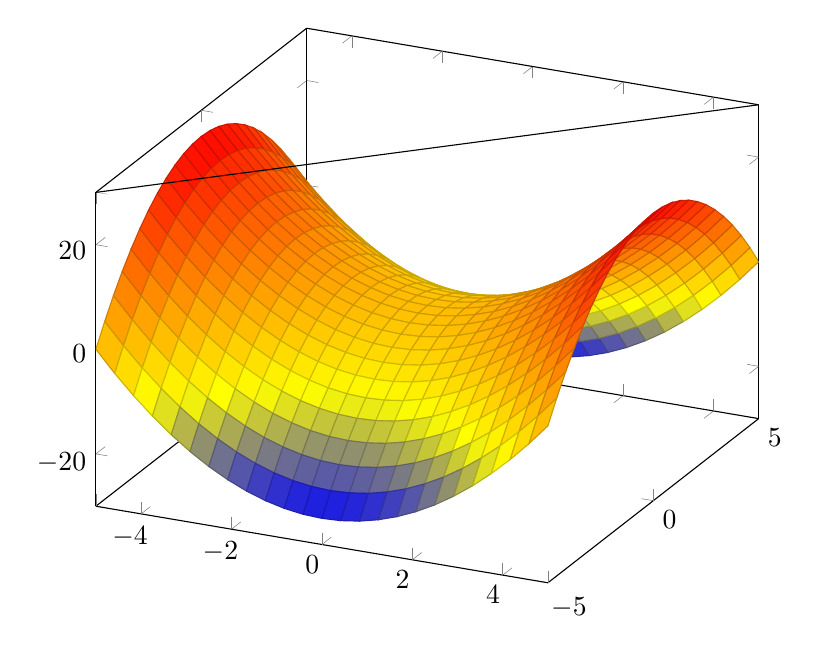
\begin{tikzpicture}
\begin{axis}
\addplot3[surf] {x^2 - y^2};
\draw (rel axis cs:0,0,1) -- (rel axis cs:1,1,1);
\end{axis}
\end{tikzpicture}

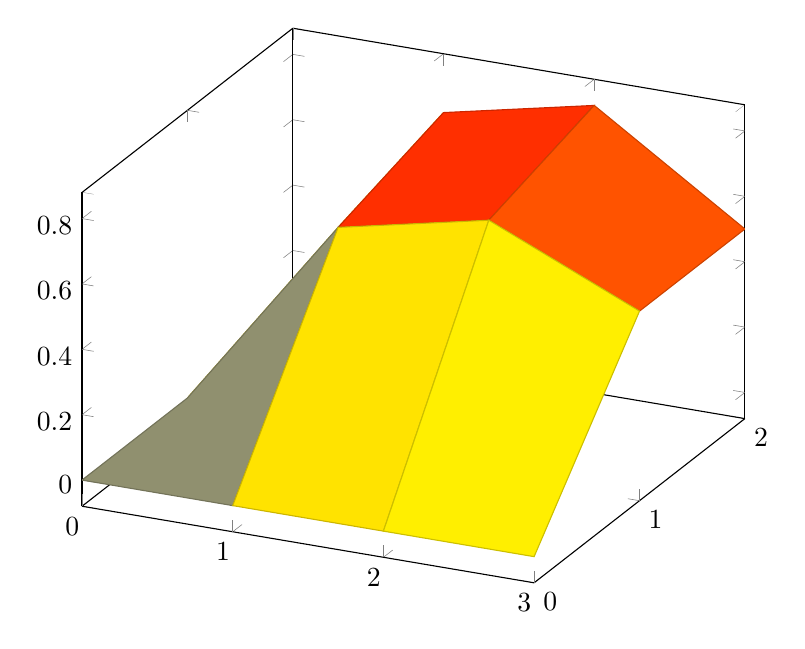
\begin{tikzpicture}
\begin{axis}
\addplot3[surf,mesh/rows=3] coordinates {
(0,0,0) (1,0,0) (2,0,0) (3,0,0)
(0,1,0) (1,1,0.6) (2,1,0.7) (3,1,0.5)
(0,2,0) (1,2,0.7) (2,2,0.8) (3,2,0.5)
};
\end{axis}
\end{tikzpicture}
\section{2D Plots}
\begin{center}
\begin{tikzpicture}
\draw[->] (-2,0) -- (2,0) node[right] {$x$};
\draw[->] (0,-2) -- (0,2) node[above] {$y$};
\draw[domain=-2:2,samples=100,blue] plot (\x, {(\x)^2 - 1});
\end{tikzpicture}
\end{center}
\end{document}
